\documentclass[a4paper,10 pt]{article}
\usepackage{geometry}
\geometry{letterpaper, margin=0.8in}
\usepackage[english]{babel}
\usepackage[utf8]{inputenc}
\usepackage{amsmath}
\usepackage{graphicx}
\usepackage[colorinlistoftodos]{todonotes}
\usepackage{float}
\usepackage[numbered]{mcode}
%\renewcommand{\baselinestretch}{1.1}
\usepackage[normalem]{ulem}
\useunder{\uline}{\ul}{}

\title{Machine Learning for Music Classification: A Test of Linear Discriminant Analysis and k-Nearest Neighbors in Three Iterations}

\author{Dana Korssjoen} 

\date{3/6/2020}

\begin{document}
\maketitle
\begin{abstract}
    This analysis applies a machine learning approach to the task of distinguishing between musical artists and genres using only computational tools. The model developed in this report uses singular value decomposition (SVD), linear discriminant analysis (PCA), and a clustering algorithm (k-nearest neighbors) to accomplish the task. The model is then tested against 3 distinct datasets, each with different structures, achieving a relatively high degree of accuracy in the best case (~80\%) and a decent degree of accuracy in the worst case (~67\%).
\end{abstract}
\section{Introduction and Overview}
One of the most interesting applications of math is trying to get computers to do things that humans can already do quite easily. I'm speaking, of course, about machine learning.

In this report, the ``thing'' that we want to teach the computer to do is to recognize music. The mathematics of the model are discussed at length in later sections, but they rely fundamentally on singular value decomposition (SVD), linear discriminant analysis (PCA), and a clustering algorithm (k-nearest neighbors). Before any learning can be done, however, an algorithm to generate the dataset of songs is developed, and these songs are transformed into their spectrograms to facilitate computation.

The particular question asked by this report is, how do different datasets respond to the algorithm developed here? Each dataset has three classes of music, and we break the datasets into 3 cases: case I, where each of the three classes contains songs from different musical artists in different genres; case II, where all three classes come from the same genre, but different artists; and case III, where the three classes come from different genres, and each class contains songs from multiple artists. In each case, we test whether the model can correctly classify samples from songs that were not included in the training data.

All of the music used in this analysis was downloaded for free from the Free Music Archive. Case I features songs from The Tudor Consort, a classical choir ensemble; Derek Clegg, a folk/acoustic artist; and King Imagine, an artist who makes electronic/ambient music. Again, all of these artists come from different genres. Case II features three artists, all from the same genre: King Imagine, as previously discussed; Livio Amato, who produces ambient/soundscape music that combines classical piano with electronic elements; and Soularflair, who produces deep electronic music. Each of these artists occupies the same genre, but there are noticeable differences in their instrumentation, rhythms, and tones. I recommend all three artists if you ever need some good studying music. Finally, case III features multiple artists within three different genres. The first genre is classical choral music; then Balkan big band (which is arguably the best genre of music in existence); and then finally, ambient/soundscape/electronic, featuring the artists from case II. I am deeply grateful to all of these artists for making their music publicly available.




\section{Theoretical Background}
\subsection{Singular Value Decomposition}
A necessary step in this analysis is transforming the data under SVD. Because this method has been discussed at length in other reports, I won't go into excessive detail; it suffices to mention that SVD can be used to extract the key components $\mathbf{U},\mathbf{\Sigma},\mathbf{V}$, and that we can capture the majority of the energy of the data using only the first several principal components. It is the this projected, reduced dataset that we will perform LDA on in the next section. We can see the share of total energy captured by each mode for the SVDs of datasets I and II in figure \ref{fig:modes}.

\subsection{Linear Discriminant Analysis}
Linear Discriminant Analysis (LDA) is a method of projecting data onto new a basis that maximizes the distance between the inter-class data while minimizing the distance between intra-class data. In simpler terms, LDA is intended to create distinct clusters of same-classed data.

Mathematically, the ideal projection $\mathbf{w}$ will take the form 
\begin{equation}
    \mathbf{w} = \arg\max_{\mathbf{w}} \frac{\mathbf{w}T\mathbf{S}_b\mathbf{w}}{\mathbf{w}^T\mathbf{S}_W\mathbf{w}}
\end{equation}
where $\mathbf{S}_b$ and $\mathbf{S}_w$ are the between-class and within-class variances, respectively, computed by
\begin{equation}
    \mathbf{S}_b = \sum_{i=1}^C (\mu_i - \mu)(\mu_i - \mu)^T
\end{equation}
and 
\begin{equation}
    \mathbf{S}_w = \sum_{i=1}^C \sum_{\mathbf{x}}(\mathbf{x}-\mu_i)(\mathbf{x}-\mu_i)^T
\end{equation}
where $C$ is the number of classes, $\mu$ is the average value across the whole dataset, and $\mu_i$ is the average value across class $i$.

Once these quantities are computed, we can find the basis $\mathbf{w}$ that achieves the desired result by solving the generalized eigenvalue problem 
\begin{equation}
    \mathbf{S}_b\mathbf{w}=\lambda\mathbf{S}_W\mathbf{w}
\end{equation}
where the maximum eigenvalue(s) $\lambda$ and the associated eigenvector(s) gives the desired projection basis. Later sections of this paper will give concrete examples of data being projected onto this basis.


\section{Algorithm Implementation and Development}
All line numbers given in this section refer to the line numbers of the MATLAB code, given in section 7, ``Appendix B: MATLAB Code.''
\subsection{Generating the Dataset}
Lines 181 - 256 generate the dataset. Not shown here (though uploaded to Github) is the set of very large matrices of urls that are used to download each individual song in each dataset. This matrix is loaded on line 186, then the minimum sampling rate for the songs in the dataset is computed by getMinFs(), which is a function that simply loops over each element of the dataset. That sampling rate is then used to downsample other songs as needed (to standardize the dataset), at which point, songs are cut into 5 second samples. Each song generates 3 samples, taken from 3 different points in the song, to increase the size of the dataset and accurately represent all features of that song.

All three datasets, as well as their labels, are then saved to be used in analysis.

Once the datasets are loaded into the main script on line 2, they are immediately split into testing and training sets with a ratio of 80/20 by the function given on lines 25-34. As seen in the results section, splitting the dataset at a specific index, rather than randomly choosing data points to be in the training set, may have introduced bias. This method was chosen consciously, however, because if data points were chosen randomly, there is extremely high probability that most of the data points would be from songs that the classifier had trained on, which would have introduced even more bias.


\subsection{Computing the Spectrograms}

Line 11 refers to a function on lines 75-92 that generate the matrix of spectrograms for the entire dataset. This is done using MATLAB's built-in spectrogram function, then unrolling each spectrogram into a column vector, so that each column of the resulting matrix is an observation from the dataset. An example signal and its spectrogram are given in figures \ref{fig:wav} and \ref{fig:spec}.

\begin{figure}
    \centering
    \begin{minipage}{0.45\textwidth}
        \centering
        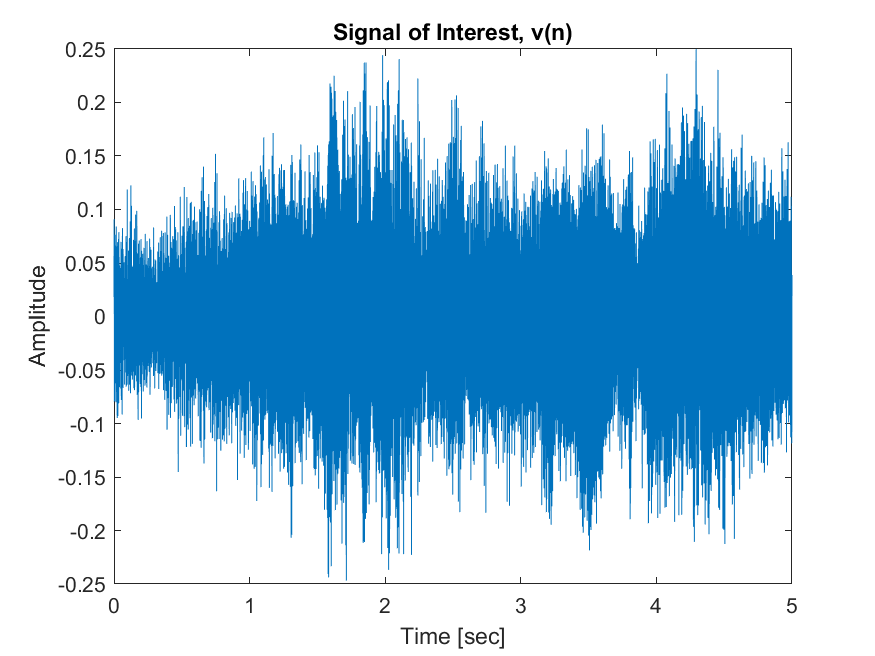
\includegraphics[width=1.15\textwidth]{hw4/wavform.png} % second figure itself
        \caption{Frequency over time of a single data point.}
        \label{fig:wav}
    \end{minipage}\hfill
    \begin{minipage}{0.45\textwidth}
        \centering
        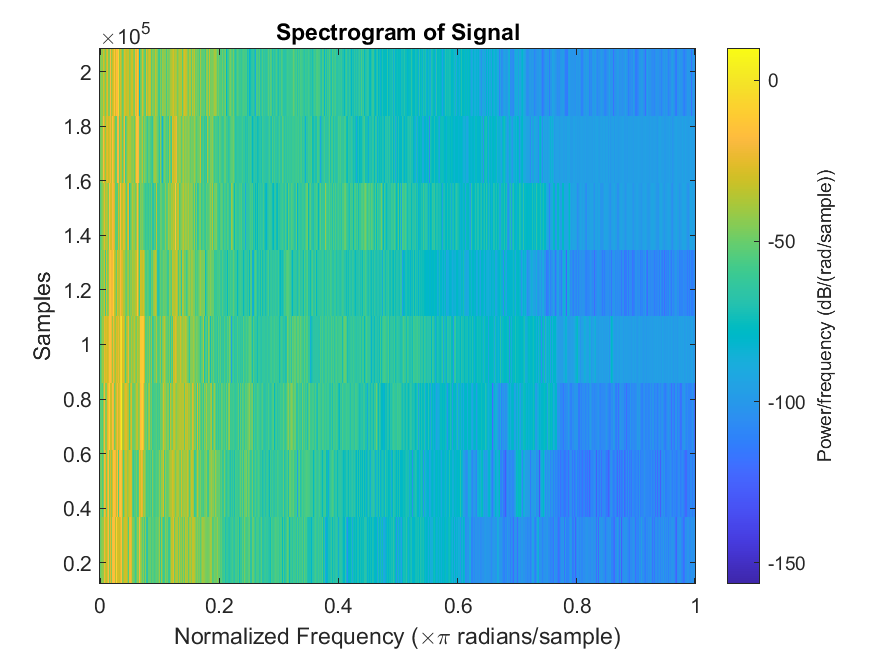
\includegraphics[width=1.15\textwidth]{hw4/spec.png} % second figure itself
        \caption{The spectrogram of that same data point.}
        \label{fig:spec}
    \end{minipage}
\end{figure}

\subsection{Linear Discriminant Analysis}

Once the spectrograms have been computed, it is time to perform LDA on line 13, which refers to a function on lines 36-73. In order to do this, the number of features is chosen based on the plots in figure \ref{fig:modes}. The number 25 was chosen because the distribution of energy among the modes is heavy-tailed, but higher numbers were found experimentally to capture too much noise and thus increase error. After the projection onto the first 25 principal components is computed, the within- and between-class variances are found. As discussed in the theoretical section, we use these to compute the best bases for our projection, hoping to maximize the distance between the means of clusters while minimizing within-class variance. The projection of the data onto these bases is returned. The results are graphed in Section 4, ``Computational Results.'' The choice to project the data into 2-dimensional, rather than 1-dimensional space was made because there is significant overlap between classes in any 1-dimensional projection.

\begin{figure}
    \centering
    \begin{minipage}{0.45\textwidth}
        \begin{figure}[H]
          \centering
            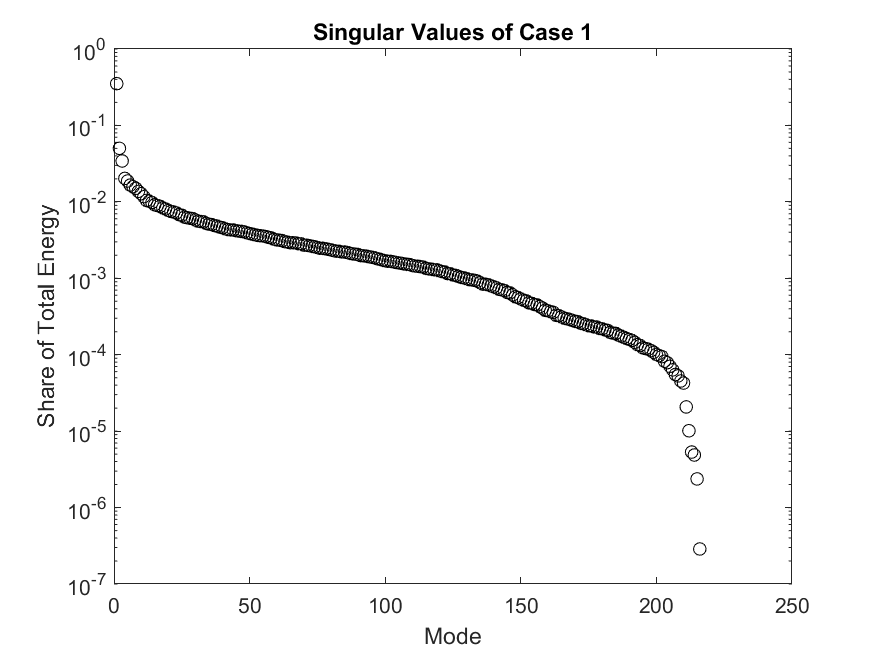
\includegraphics[width = 1.15\textwidth]{hw4/modes-1.png}
        \end{figure}
    \end{minipage}\hfill
    \begin{minipage}{0.45\textwidth}
        \begin{figure}[H]
          \centering
            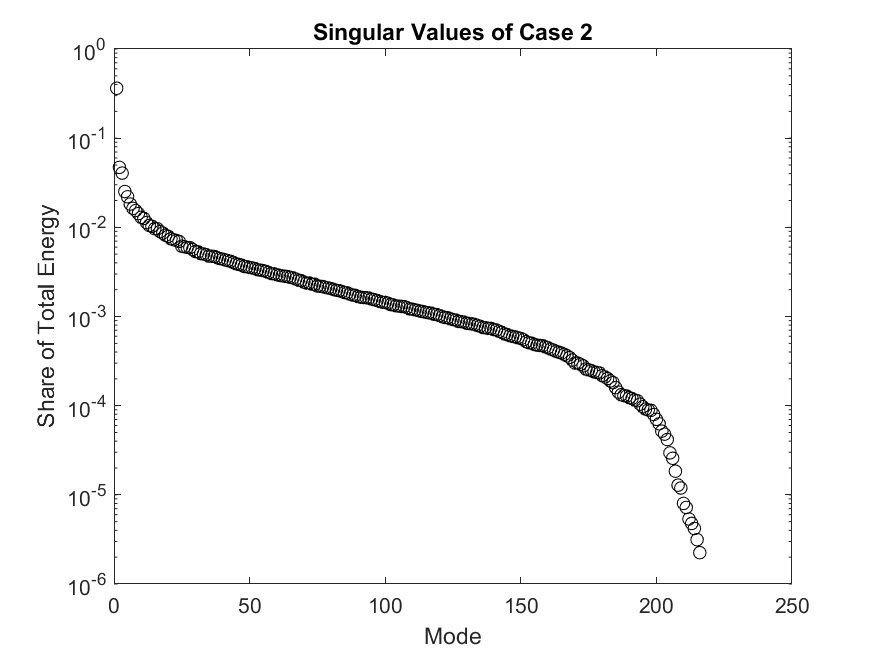
\includegraphics[width = 1.15\textwidth]{hw4/modes-2.png}
        \end{figure}
    \end{minipage}
    \caption{Energy of the singular values of case I (left) data and case II (right) data. Energy is depicted as the share of total energy represented by that mode.}
    \label{fig:modes}
\end{figure}




\subsection{Classification}

Finally, classification of the projected test data is performed using the popular k-nearest neighbors (KNN) algorithm, which is called on line 18 and written on lines 94-106. This algorithm finds the $k$ nearest labelled points to the given unlabelled points, then predicts that the mystery point has the mode (most frequent) of their labels. If there is a tie for which labels appears with the highest frequency, the label which is closest to the point is predicted. The value $k=5$ was selected experimentally. We can anticipate that KNN is an appropriate classification algorithm for this data set, because our intention with LDA was to group each point into the most homogenous same-classed clusters are possible, and to maximize the distance between clusters. Thus, we would ideally anticipate the nearest neighbors of any given point, would be points in the same class. This idea is confirmed by our relatively low error rate, as discussed in the following section.




\section{Computational Results}

Figures \ref{fig:scat-test-1} and \ref{fig:scat-err-1} depict the LDA projection of the data from case I. In figure \ref{fig:scat-test-1}, only the testing data (with the hidden labels) is projected, and in figure \ref{fig:scat-err-1}, all training data, plus the testing data which was mislabelled by the classifier is projected. In table \ref{tab:err-1}, the predicted vs actual classes of the 11 mislabelled testing points are included. As can be seen in the table, many data points from class 3 were mislabelled. In figures \ref{fig:scat-test-1} and \ref{fig:scat-err-1} we can see why this might be the case, as many of the mislabelled class 3 points are confoundingly close to the class 1 cluster. In fact, it appears that the testing points for class 3 are distributed differently than the training points, which suggests there may have been error in the way the dataset was constructed, interference from the relatively small number of data points, or error resulting from the sampling method.


\begin{figure}
    \centering
    \begin{minipage}{0.45\textwidth}
        \centering
        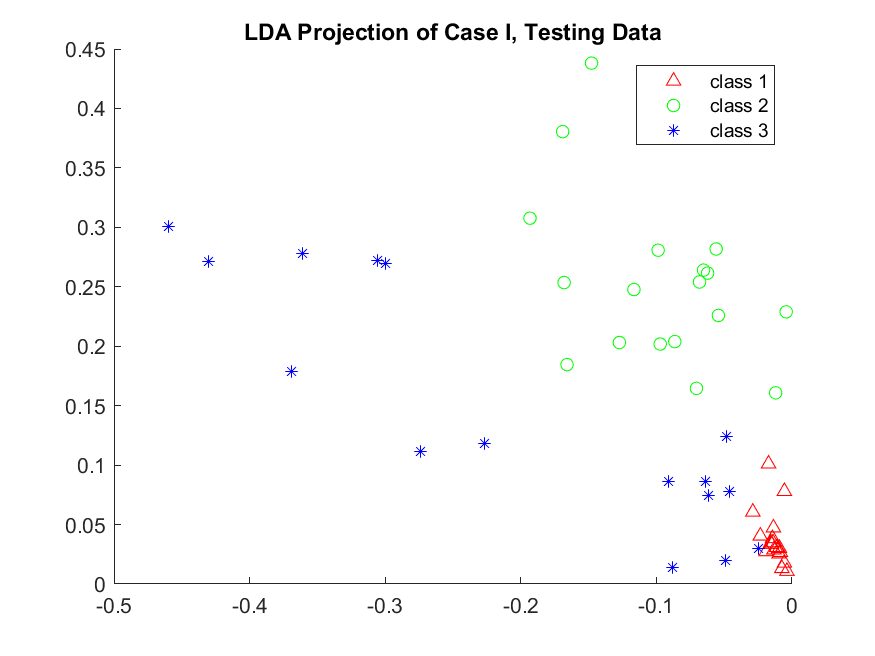
\includegraphics[width=1.15\textwidth]{hw4/scat-test-1.png} % second figure itself
        \caption{Testing data from case I}
        \label{fig:scat-test-1}
    \end{minipage}\hfill
    \begin{minipage}{0.45\textwidth}
        \centering
        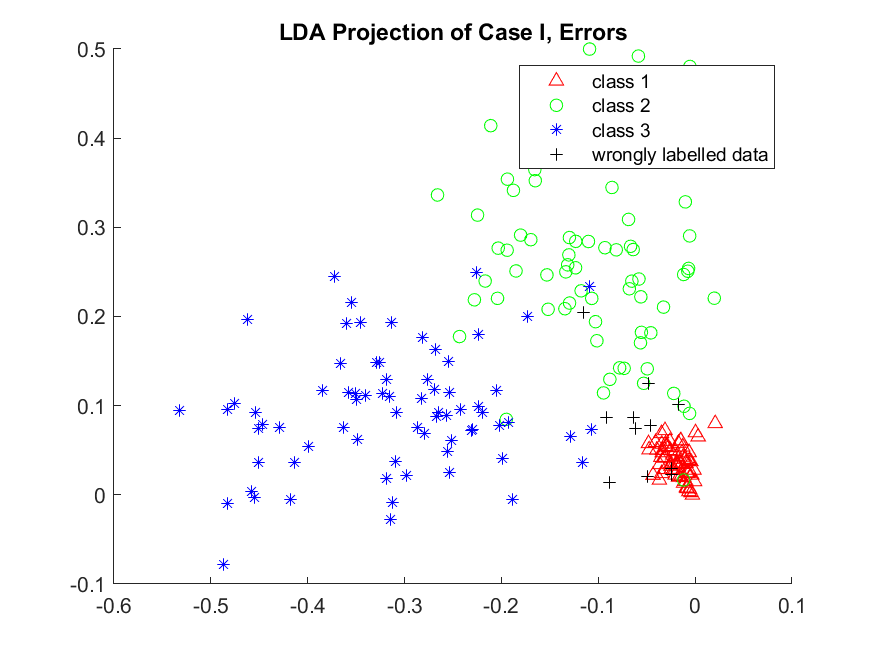
\includegraphics[width=1.15\textwidth]{hw4/scat-err-1.png} % second figure itself
        \caption{Mislabelled testing data from case I}
        \label{fig:scat-err-1}
    \end{minipage}
\end{figure}

\begin{table}[]
\centering
\begin{tabular}{|l|l|l|l|l|l|l|l|l|l|l|l|}
\hline
Predicted & 2 & 1 & 1 & 1 & 1 & 2 & 1 & 2 & 1 & 2 & 1 \\ \hline
Actual & 1 & 3 & 3 & 3 & 3 & 3 & 3 & 3 & 3 & 3 & 3 \\ \hline
\end{tabular}
\caption{Mislabelled points in case I dataset.}
\label{tab:err-1}
\end{table}


Analogous figures for case II are included as figures \ref{fig:scat-test-2} and \ref{fig:scat-err-2}, and table \ref{tab:err-2} depicts the 18 mislabelled testing points. As in case I, the errors in case II seems to come from the fact that the testing data for case II is distributed differently that the training data, particularly for class 1, where we saw the most errors. The reasons for this are discussed above. Intuitively, it makes sense that this case had more error than case I, however, because the degree of difference between bands in the same genre is typically much smaller than that between bands in different genres. Understandably, then, our classifier had more difficulty distinguishing between bands.

\begin{figure}
    \centering
    \begin{minipage}{0.45\textwidth}
        \centering
        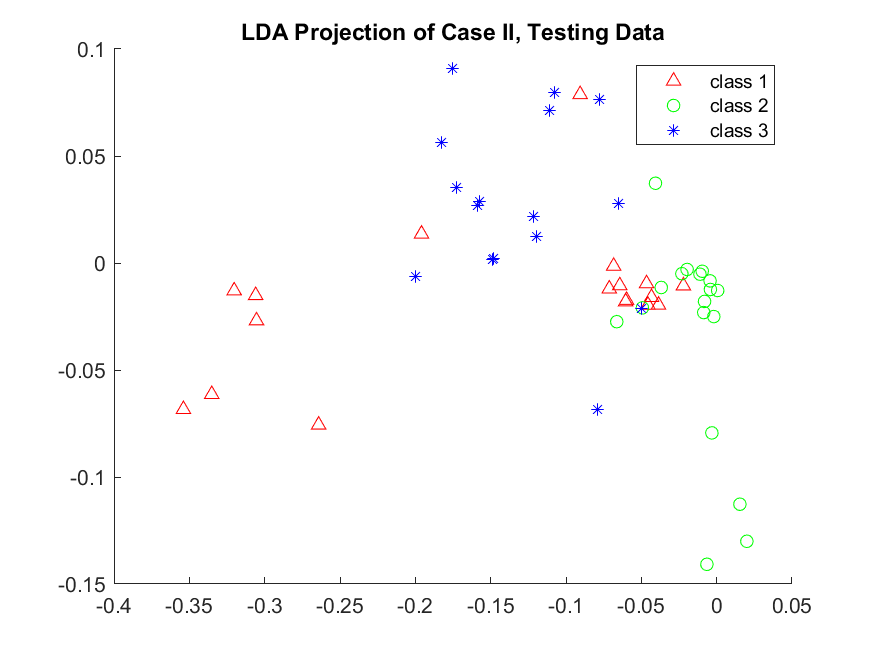
\includegraphics[width=1.15\textwidth]{hw4/scat-test-2.png} % second figure itself
        \caption{Testing data from case II}
        \label{fig:scat-test-2}
    \end{minipage}\hfill
    \begin{minipage}{0.45\textwidth}
        \centering
        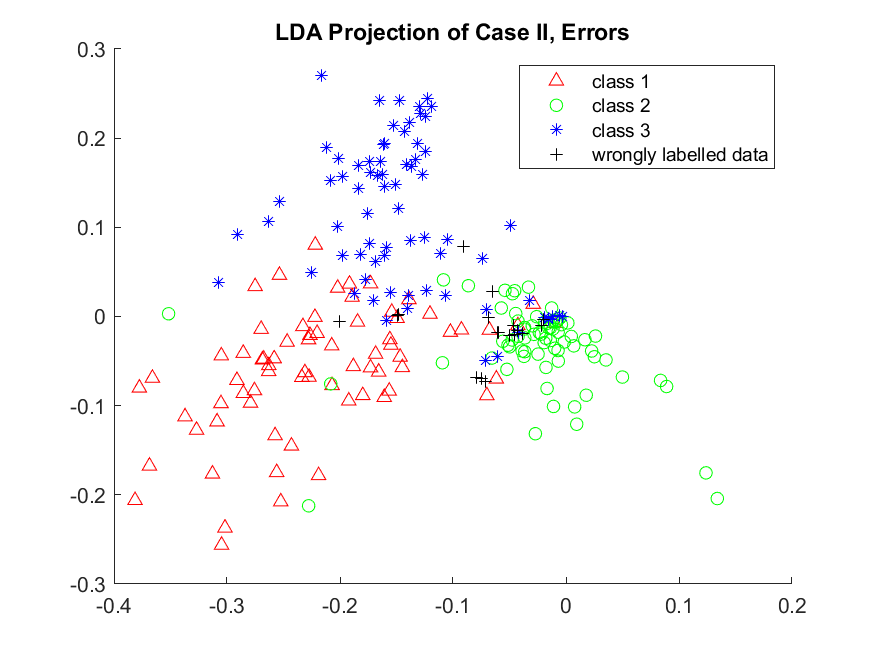
\includegraphics[width=1.15\textwidth]{hw4/scat-err-2.png} % second figure itself
        \caption{Mislabelled testing data from case II}
        \label{fig:scat-err-2}
    \end{minipage}
\end{figure}

\begin{table}[]
\centering
\begin{tabular}{|l|l|l|l|l|l|l|l|l|l|l|l|l|l|l|l|l|l|l|}
\hline
Predicted & 2 & 2 & 2 & 2 & 2 & 2 & 2 & 2 & 2 & 2 & 2 & 2 & 1 & 1 & 1 & 1 & 1 & 1 \\ \hline
Actual & 1 & 1 & 1 & 1 & 1 & 1 & 1 & 1 & 1 & 2 & 3 & 3 & 3 & 3 & 3 & 3 & 3 & 3 \\ \hline
\end{tabular}
\caption{Mislabelled points in case II dataset.}
\label{tab:err-2}
\end{table}

The results for case III are included as figures \ref{fig:scat-test-3} and \ref{fig:scat-err-3}, and table \ref{tab:err-3} depicts the 12 mislabelled testing points. This case had particular trouble with samples from class 1, which have high variance in the testing data. The same factors as before may have influenced. Despite that, however, we achieved a relatively equal degree of accuracy between cases I and III. Again, this is likely due to that fact that different genres can have vastly different musical characteristics, so the means between the classes would naturally be farther away from one another. Compare this to case II, where same-genre bands are expected to be more similar musically. Note that we cannot conclusively say whether our classifier was more successful with case I or case III, since their total errors was only off by one, which suggests that the more salient feature in our model was which genre a song was from, not which specific musical artist.

All told, the error rate for case I was 11/54, or 20\%; for case II was 18/54, or 33\%; and for case III was 12/54, or 22\%.

\begin{figure}
    \centering
    \begin{minipage}{0.45\textwidth}
        \centering
        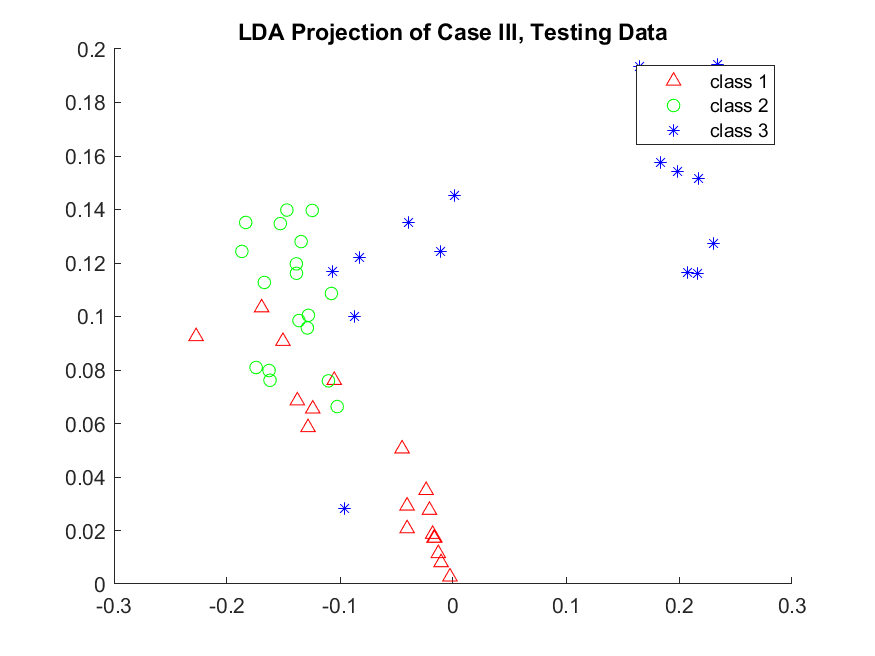
\includegraphics[width=1.15\textwidth]{hw4/scat-test-3.png} % second figure itself
        \caption{Testing data from case III}
        \label{fig:scat-test-3}
    \end{minipage}\hfill
    \begin{minipage}{0.45\textwidth}
        \centering
        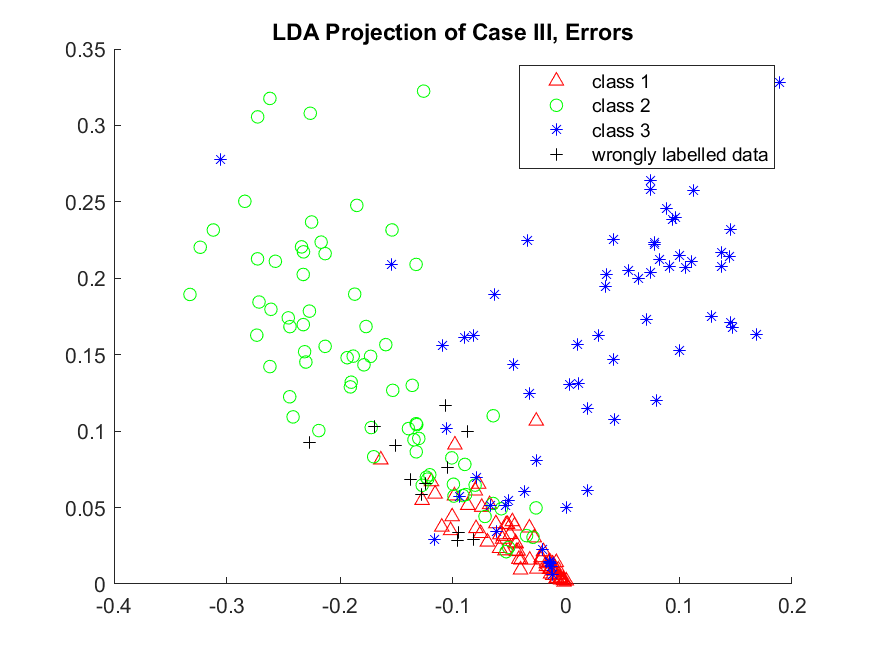
\includegraphics[width=1.15\textwidth]{hw4/scat-err-3.png} % second figure itself
        \caption{Mislabelled testing data from case III}
        \label{fig:scat-err-3}
    \end{minipage}
\end{figure}

\begin{table}[]
\centering
\begin{tabular}{|l|l|l|l|l|l|l|l|l|l|l|l|l|}
\hline
Predicted & 2 & 2 & 2 & 2 & 2 & 2 & 2 & 2 & 2 & 1 & 1 & 1 \\ \hline
Actual & 1 & 1 & 1 & 1 & 1 & 1 & 1 & 3 & 3 & 3 & 3 & 3 \\ \hline
\end{tabular}
\caption{Mislabelled points in case III dataset.}
\label{tab:err-3}
\end{table}


\section{Summary and Conclusions}
As discussed in the computational results section, we may tentatively conclude that the model used in this paper is more equipped to distinguish between genres than between musical artists. There is something that we can conclude confidently, however -- the fact that a simple series of mathematical transformations enabled a computer to (somewhat) reliably ``recognize'' music. The potential applications for this technique, and techniques like it, are profound, particularly if one were to heed the lessons learned in this report by ensuring that datasets are sufficiently large, and training data is obtained in a randomized way in order to minimize error in applications. 
\section{Appendix A: MATLAB Functions and Implementation}
See table \ref{tab:functions}, which appears underneath the heading for the following section because LaTeX is \emph{very} confusing.
\begin{table}[]
\begin{tabular}{ll}
\textbf{Function} & \textbf{Implementation} \\
load(A) & loads the file or data given by A into the workspace \\
nnz(A) & returns the number of non-zero elements in A \\
length(A) & returns the length of vector A \\
svd(A) & performs a singular value decomposition on A \\
mean(A, dim) & computes the mean of A along dimension dim \\
eig(A,B) & finds the solution to the generalized eigenvalue problem described by A and B \\
maxk(A,k) & finds the k maximum entries in A \\
size(A,dim) & returns the size of A along dimension dim \\
spectrogram(A) & computes the spectrogram of A; plots it if output is not supressed by semicolon \\
zeros(n,m) & returns an nxm matrix of all zeros \\
abs(A) & returns the absolute value of A \\
reshape(A, {[}n m{]}) & reshapes A into an nxm matrix \\
repmat(A, n, m) & replicates matrix A to construct a new matrix of shape nxm \\
mode(A, dim) & returns the mode of A along dimension dim \\
webread(A) & reads content from RESTful web service; returns as data \\
downsample(A, n) & downsamples A by a factor of n
\end{tabular}
\label{tab:functions}
\end{table}
\section{Appendix B: MATLAB Code}
\begin{lstlisting}
%% load & split data
load('songs.mat')
[Atr,Ats,Ltr,Lts] = split_train_test(A,lab);

%% main body - run this for each dataset
X = A; % edit only this line to change dataset

% split data
[Xtr,Xts,Ltr,Lts] = split_train_test(X,lab);
% make specs
Xsp = spec_vec(Xtr);
% make projection
[Xtr,U,S,w] = LDA2(Xsp,25,90*.8);
% apply to test data
Xtssp = spec_vec(Xts);
Xts = w'*(U'*Xtssp);
% knn
plab = knn(Xtr,Ltr,Xts,5);
% calculate error
errs = nnz(plab-Lts);
err_ind = plab~=Lts;
err_rate = errs/length(plab);

%% functions
% assumption: obs need to be columns in A
function [Atr,Ats,Ltr,Lts] = split_train_test(A,lab)
    % save 18 out of every 90 for testing (20%)
    train = 1:72;
    test = 73:90;
    Atr = [A(:,train) A(:,train+90) A(:,train+180)];
    Ltr = [lab(train) lab(train+90) lab(train+180)];
    Ats = [A(:,test) A(:,test+90) A(:,test+180)];
    Lts = [lab(test) lab(test+90) lab(test+180)];
end

% LDA2: 2 for 2-dim projection
% n is num of each class in the data - classes MUST be consecutive
function [result,U,S,w] = LDA2(X, feature,n)
    
    [U,S,V] = svd(X,'econ');
    Xp = S*V'; % proj onto principal components
    U = U(:,1:feature);
    X1 = Xp(1:feature,1:n);
    X2 = Xp(1:feature,(n+1):(2*n));
    X3 = Xp(1:feature,(2*n+1):(3*n));
    
    % calculate Sw,Sb
    m1 = mean(X1,2);
    m2 = mean(X2,2);
    m3 = mean(X3,2);
    Sw = 0; % within class
    for i=1:n
        Sw = Sw + (X1(:,i)-m1)*(X1(:,i)-m1)';
        Sw = Sw + (X2(:,i)-m2)*(X2(:,i)-m2)';
        Sw = Sw + (X3(:,i)-m3)*(X3(:,i)-m3)';
    end
    m = (m1+m2+m3)/3;
    Sb1 = (m1-m)*(m1-m)'; % between class
    Sb2 = (m2-m)*(m2-m)';
    Sb3 = (m3-m)*(m3-m)';
    Sb = Sb1+Sb2+Sb3;
    
    % LDA
    [V2,D] = eig(Sb,Sw);
    [lambda,I] = maxk(abs(diag(D)),2);
    w1 = V2(:,I(1)); %w1 = w1/norm(w1,2);
    w2 = V2(:,I(2)); %w2 = w2/norm(w2,2);
    
    % 2-dim proj
    w = [w1 w2];
    v1 = w'*X1; v2 = w'*X2; v3 = w'*X3;
    result = [v1,v2,v3];
end

% make specs
% X must have observations as cols
function [spec] = spec_vec(X)
    n = size(X,2); % num of observations

    % determine size for memory pre-allocation
    tmp = spectrogram(X(:,1));
    sz = size(tmp);
    
    % make spectrogram matrix
    spec = zeros(sz(1)*sz(2),n);
    for j=1:n
        s = spectrogram(X(:,j));
        s = abs(s);
        s = reshape(s, [sz(1)*sz(2),1]);
        spec(:,j) = s;
    end
end

% knn
function [pred] = knn(tr,lab,ts,k)
    ntr = size(tr,2);
    nts = size(ts,2);
    X = repmat(ts(1,:),ntr,1)-repmat(tr(1,:)',1,nts);
    Y = repmat(ts(2,:),ntr,1)-repmat(tr(2,:)',1,nts);
    l2 = (X.^2 + Y.^2).^(1/2); % Euclid. dist
    
    % for each col, find k least entries
    [~,I] = sort(l2,1);
    pred = lab(I(1:k,:));
    pred = mode(pred,1); % takes 1st sorted item for ties
end

%% below code is plotting & data generation - reading it is not necessary in order to 
% understand the methods used in this analysis

%% plotting
%% one-time plots
% example wavform
v=A(:,1)'; Fs = 44100;
plot((1:length(v))/Fs,v);
xlabel('Time [sec]');
ylabel('Amplitude');
title('Signal of Interest, v(n)');
xlim([0 5]);
saveas(gcf,'wavform.png')

close all;
% example spec
spectrogram(v);
title('Spectrogram of Signal');
saveas(gcf,'spec.png')

%% plots for all cases
% scatter, training data
close all;
scatter(Xtr(1,1:71),Xtr(2,1:71),'^r')
hold on
scatter(Xtr(1,72:143),Xtr(2,72:143),'og')
scatter(Xtr(1,144:216),Xtr(2,144:216),'*b')
legend('class 1','class 2','class 3')
title('LDA Projection of Case I, Training Data');
saveas(gcf,'scat-train-1.png')

close all;
% scatter, testing data
scatter(Xts(1,1:18),Xts(2,1:18),'^r')
hold on
scatter(Xts(1,19:36),Xts(2,19:36),'og')
scatter(Xts(1,37:52),Xts(2,37:52),'*b')
legend('class 1','class 2','class 3')
title('LDA Projection of Case I, Testing Data');
saveas(gcf,'scat-test-1.png')

close all;
% scatter, all data
scatter(Xtr(1,1:71),Xtr(2,1:71),'^r')
hold on
scatter(Xtr(1,72:143),Xtr(2,72:143),'og')
scatter(Xtr(1,144:216),Xtr(2,144:216),'*b')
scatter(Xts(1,:),Xts(2,:),'+k')
legend('class 1','class 2','class 3','testing data')
title('LDA Projection of Case I, All Data');
saveas(gcf,'scat-all-1.png')

close all;
% scatter, errors + training data
err_pts = [plab(err_ind); Lts(err_ind)];
scatter(Xtr(1,1:71),Xtr(2,1:71),'^r')
hold on
scatter(Xtr(1,72:143),Xtr(2,72:143),'og')
scatter(Xtr(1,144:216),Xtr(2,144:216),'*b')
scatter(Xts(1,err_ind),Xts(2,err_ind),'+k');
legend('class 1','class 2','class 3','wrongly labelled data')
title('LDA Projection of Case I, Errors');
saveas(gcf,'scat-err-1.png')

close all;
% energy vs mode
lambda = diag(S).^2;
semilogy(lambda/sum(lambda),'ko')
xlabel('Mode')
ylabel('Share of Total Energy')
title('Singular Values of Case 1')
saveas(gcf,'modes-1.png')

%% data generation
% urls.mat, the script for creating the matrices of urls, is not included here for brevity 
% (it's over 200 lines long), but it is uploaded to github

%% get_data.m
load('urls.mat')

% make labels
m = zeros(1,90);
lab = [m+1 m+2 m+3];

mFs = getMinFs(Au);
A = [];
for j=1:size(Au,1) 
    [y,Fs] = webread(Au(j,1));
    % stereo -> mono
    if size(y,2)==2
        y = (y(:,1)+y(:,2))/2;
    end
    y = downsample(y, round(Fs/mFs));
    % take 3 samples, (roughly) 5 sec each
    A = [A; 
        y(30*mFs:35*mFs,:)';
        y(45*mFs:50*mFs,:)';
        y(60*mFs:65*mFs,:)'];
end

mFs = getMinFs(Bu);
B = [];
for j=87:size(Bu,1) 
    [y,Fs] = webread(Bu(j,1));
    % stereo -> mono
    if size(y,2)==2
        y = (y(:,1)+y(:,2))/2;
    end
    % downsample
    y = downsample(y, round(Fs/mFs));
    Fs = Fs/2;
    % take 3 samples, 5 sec each
    B = [B; 
        y(30*mFs:35*mFs,:)';
        y(45*mFs:50*mFs,:)';
        y(60*mFs:65*mFs,:)'];
end

mFs = getMinFs(Cu);
C = [];
for j=1:size(Cu,1) 
    [y,Fs] = webread(Cu(j,1));
    % stereo -> mono
    if size(y,2)==2
        y = (y(:,1)+y(:,2))/2;
    end
    % downsample
    y = downsample(y, round(Fs/mFs));
    Fs = Fs/2;
    % take 3 samples, 5 sec each
    C = [C; 
        y(30*mFs:35*mFs,:)';
        y(45*mFs:50*mFs,:)';
        y(60*mFs:65*mFs,:)'];
end

A = A'; B = B'; C = C'; % each col is a song now
Fs=mFs;
save('data.mat','A','B','C','lab','Fs')

function [minFs] = getMinFs(U)
    [~,minFs] = webread(U(1));
    for j=2:size(U,1)
        [~,Fs] = webread(U(j));
        if Fs < minFs
            minFs = Fs;
        end
    end
end

\end{lstlisting}
\end{document}